\subsubsection{Monitoraggio e Valutazione}
Quando vedete una freccia circolare bisogna pensare al \textbf{PDCA} (Plan Do
Check Act). Infatti, ormai tutti i progetti sono circolari. \emph{Kaizen} è
una parola giapponese che vuol dire “miglioramento continuo”. Quando si vede
che c’è un delta, ovvero uno scostamento tra valore atteso e valore ottenuto,
si cerca di operare per migliorarlo. Una volta raggiunti gli obiettivi
prefissati, come previsto dal \textbf{PDCA}, bisogna fissare dei nuovi
obiettivi da raggiungere per migliorarsi continuamente.

\begin{itemize}
\item ME1: monitorare e valutare le prestazioni dell'IT;
\item ME2: monitorare e valutare i controlli interni;
\item ME3: assicurare la conformità a leggi e normative esterne;
\item ME4: istituire l'IT governance.
\end{itemize}

Sulla nuova normativa di privacy se l'azienda non intraprenderà le procedure
adeguate per preservare la privacy, avrà delle multe fino al 5\% del fatturato
e la possibilità di andare a processo.

\subsubsection{SSE-CMM: System Security Engineering Capability Maturity Model}

Modelli di maturità. Questa categorizzazione si applica a tutto. Nata per
l'ingegneria del Software.
La maturità è la capacità di governare i processi: se si riesce anche a
mettere in pratica il miglioramento continuo si è a livelli alti.

Di conseguenza, gli investitori saranno più portati a investire in aziende che
hanno un CMM alto rispetto a uno basso, in quanto le aziende con
un CMM basso (dallo Stage 2
in giù) sono fortemente legate al lato ``umano''. 
Essere a livelli alti è anche un vantaggio che si può portare sul 
mercato.

Grazie a questo è possibile mettere in piedi un sistema di miglioramento
continuo.

\begin{figure}[h!]
        \begin{center}
                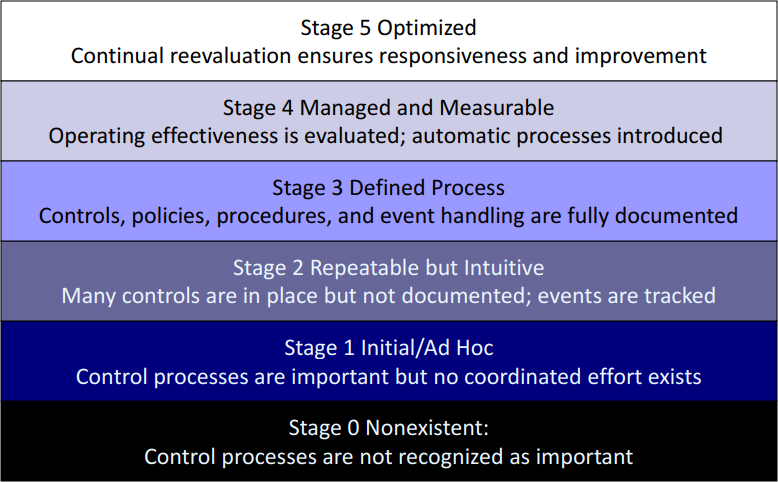
\includegraphics[scale=2.0]{res/img/maturity_level}
        \end{center}
        \caption{I 5 livelli del Capability Maturity Model (CMM).}
        \label{fig:cmm:levels}
\end{figure}

Se i controlli non sono documentati non si sa come possono essere migliorati,
valutati, ecc\dots

\emph{I livelli sono molto importanti:} dal Livello 4 in su,
l'automatizzazione dei processi di controllo permette un risparmio sul TCO
(Total Cost of Ownership).



\subsubsection{Standard di sicurezza}

ISO 27001 e il COBIT sono gli standard di sicurezza di base. La \textit{gap
analysis} (differenza tra dove vorremmo essere e dove siamo) ci aiuta a capire
dove sono presenti le lacune da colmare.

\begin{figure}[h!]
        \begin{center}
                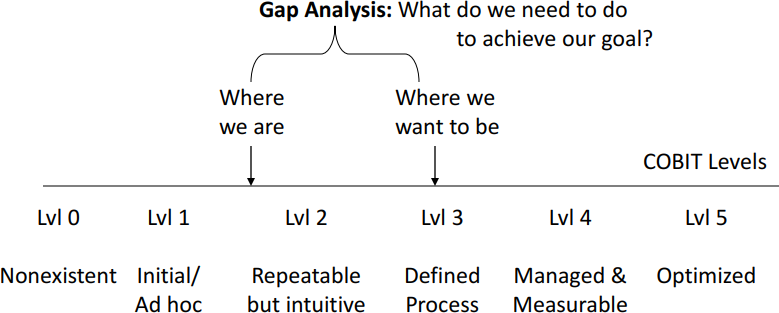
\includegraphics[scale=2.0]{res/img/security_standard}
        \end{center}
        \caption{I 5 livelli del Capability Maturity Model (CMM) e il
        loro rapporto con un programma di sicurezza.}
\end{figure}


\subsubsection{Esercizi}

Gli esercizi sono disponibili in \ref{esSM:COBIT}

\chapter{Policy and Governance}
\label{PG}

\section{Governance}

\textbf{Corporate governance:} è la leadership da parte dei direttori
aziendali nel creare e presentare il valore agli stakeholders.\\
\newline
\textbf{IT governance:} si assicura del corretto allineamento dell'IT con gli
obiettivi aziendali.



\section{Strategic Planning Process}
\label{PG:SPP}

Oggi come oggi una \textbf{pianificazione strategica} nell'IT è in 3 anni, in
quanto tra 5 anni nessuno sa cosa ci sarà. Quindi la lunghezza dei piani si è
accorciata, specialmente nel settore informatico in quanto la pressione
tecnologica è altissima. Questa pianificazione è destinata ad accorciarsi
grazie all'intelligenza artificiale, che aiuterà gli umani a prendere
decisioni. La \textbf{pianificazione tattica} dura un anno e permette
all'organizzazione di muoversi verso gli obiettivi strategici, mentre la
\textbf{pianificazione operazionale} definisce piani dettagliati o tecnici.

\begin{figure}[H]
        \begin{center}
                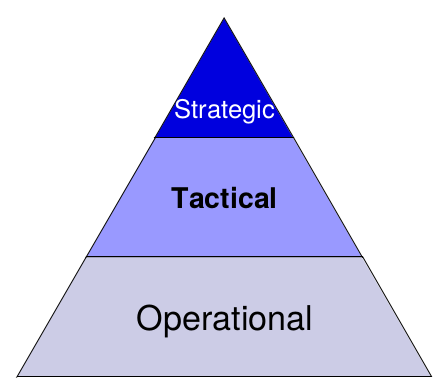
\includegraphics[scale=0.4]{res/img/planning_process}
        \end{center}
        \caption{Piramide dei differenti tipi di pianificazione.}
\end{figure}

